\section{OpenStack Customizations for NFV}

Virtualization provides flexibility and scalaility of resources by enabling the workloads to be run on virtual machines that can be migrated, replicated and restarted quickly. However, the virtual machines still need to share the physical hardware resources like CPU, Memory and I/O. This results in significant performance penalties on the workloads. Use-cases for NFV require consistent performance and many times require real-time capabilities. To achieve this, tuning the operating system and I/O mechanisms would be necessary. The tuning can involve simple toggling of operating system features or introduction of a different library and driver along with hardware customizations to achieve the desired result.

\begin{enumerate}

\item Tuning Compute Performance

\begin{flushleft}
Through filtered scheduler available in Nova, OpenStack provides ability to tune Compute performance for intensive workloads that run within the Vms. This is done by enabling features such as CPU Pinning, Huge-Pages and NUMA-Affinity through configurations set in Nova during deployment. This will ensure that the selected nodes for provisioning or migrating the VM has the relevant features enabled. These parameters are available for tuning in most current operating systems and therefore do not need any special component to achieve the performance expectations for these parameters.
\end{flushleft}

\item Tuning Network I/O Performance

\begin{flushleft}
Network I/O performance is critical for the type of actions that NFV use-cases expect to perform on the VNFs. It demands fast inter-VM communication both within and across the compute nodes. 
The network architecture of the OpenStack uses the separation concept proposed by SDN technologies. The control plane is usually implemented as part of the Network services that run on the OpenStack Controller or dedicated Network node as the case may be. The data plane can be implemented either through direct connection to the NICs or through bridging allowing for multiple Vms to be hosted on a single node. We discuss the following approaches for data plane methods:
\end{flushleft}
		
    \begin{itemize}
        \item Linux Bridge
            This is the traditional Linux networking implementation provided by linux-utils and provides a simple interface to provide multiple interfaces on a single NIC\@. The linux bridge is inherently slow and the limits on the number of interfaces make it non-viable for scalability. A typical connectivity in a Linux bridge network is as in the figure below [5].
            \begin{figure}[h!]
		        \centering
  		        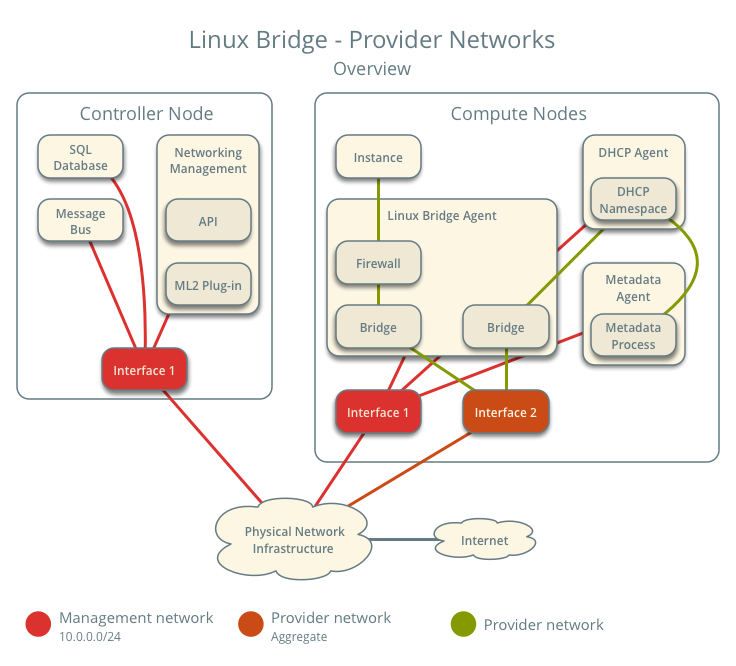
\includegraphics[width=0.9\textwidth]{linux_bridge_provider}
  		        \label{fig:figure12}
		        \caption{OpenStack Network with Linux Bridge Provider Network}
	        \end{figure}
        \item OpenvSwitch
            OpenvSwitch provides a virtual switching mechanism and is based on OpenFlow Protocol. 
            \begin{figure}[h!]
		        \centering
                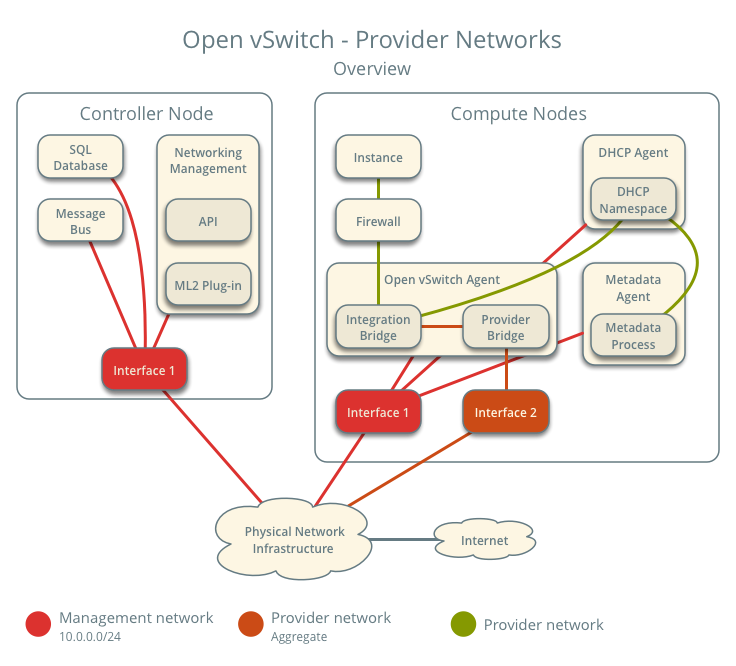
\includegraphics[width=0.9\textwidth]{ovs_provider}
		        \label{fig:16}
		        \caption{OpenStack Network with OpenVswitch as the Provider Network}
	        \end{figure}
            The multiple levels of bridging in the OpenvSwitch based architecture creates performance bottlenecks that hinder the use-cases for NFV\@. Hence advanced data plane acceleration technologies should be utilized. The key data plane acceleration methods are listed below.
	
        \item DPDK - Data Plane Development Kit
	    \item VPP - Vector Packet Processing
	    \item SRIOV - Single Root I/O Virtualization
    \end{itemize}			
\end{enumerate}
